\chapter{Shape Detection}
\section{Overview}
The shape detection runs automatically in the background. It is designed such that the user receives imminent feedback of local geometry for the region under the mouse cursor. The approach utilizes an automated shape detection algorithm that is capable of detecting different types of primitive shapes. This algorithm is designed to find shapes in point clouds that consist of several million points within minutes. However, when looking at the performance for smaller samples, results can be achieved at interactive time rates. 
Section \ref{sec:schnabel} describes the shape detection algorithm. 
Shape detection is performed one small regions at once. Section \ref{sec:candidateNodes} describes a heuristic on how to choose such a region using the user's cursor position and view as input. This efficiently changes the usecase from an automated shape detection to a user-controlled shape detection. 
In order to use the detected shapes for rendering and interactions, the shapes must be postprocessed. 
Since some of the shapes are of infinite size the, those shapes need to be refitted to fit the corresponding support points. Section\ref{sec:Refitting} goes into detail for each shape. 

\section{Efficient RANSAC for Point-Cloud Shape Detection}
\label{sec:schnabel}
The section gives a brief overview over the algorithm used to detect primitive shapes. 
Schnabel et. al\cite{schnabel-2007-efficient} propose an automated way for detecting simple primitive shapes in unstructured point clouds. The point cloud is decomposed into a set of shapes and a set unused points. The algorithm supports detection of planes, spheres, cylinders, cones, and tori. 

\textbf{RAN}dom \textbf{SA}mpling \textbf{C}onsens (RANSAC) was first discussed by Fischler and Bolles\cite{fischler1981random} as a paradigm for model fitting for image analysis and automated cartography. However, this approach can be generalized for points with an origin other than images. The shape detection utilizes RANSAC to repeatedly take a minimal set of points to build a primitive shape $\Psi$ and checks if the points in the region roughly follow the curvature of the shape. 

\subsection{Minimal sets}
A minimal set describes the set of points that is needed to construct a candidate shape. 
For each type of shape the following rule applies: A shape is only considered as candidate shape if all points from the minimal set are within a distance $\epsilon$ to the shape and the normal does not deviate from the shape's normal by more than an angle $\alpha$. 

\begin{itemize}
	\item \textbf{Plane}: A plane is constructed from three points $p_0, p_1, p_2$ whose normals do deviate from the plane's normal less than the angle $\alpha$. 
	
	\item \textbf{Sphere}: A sphere is fully defined by two points $p_0, p_1$ with corresponding normal vectors $n_0, n_1$. The center $c$ of the sphere is defined by the midpoint shortest line segment between the parametric lines $p_0 + tn_0$ and $p_1 + sn_1$. The radius is constructed by averaging the distance of $p_0$ and $p1$ to $c$.

	\item \textbf{Cylinder}:
	In order to create a cylinder a minimal set of two points  $p_0, p_1$ with corresponding normal vectors $n_0, n_1$ is used. The direction $d$ of the axis is established by $d = n_0 \times n_1$. The origin $c$ of the cylinder is created by projecting the parametric lines $p_0 + tn_0$ and $p_1 + sn_1$ onto the plane $d \cdot x = 0$ and taking their intersection as origin $c$. The radius is the shortest distance between $p_0$ and the axis $c + ud$
	
	\item \textbf{Cone}:
	For simplicity, an cone the minimal set for a cone consists of three points $p_0, p_1, p_2$, rather than two. From each point-normal pair a plane is created. The intersection of the three planes defines the apex $c$. To describe the direction of the axis a plane is constructed from the points \{$c +  \frac{p_0 - c}{||p_0 - c||}$, $c +  \frac{p_1 - c}{||p_1 - c||}$, $c +  \frac{p_2 - c}{||p_2 - c||}$\}. The normal of this plane is the direction $d$ of the cone axis. The opening angle is given as $\omega = \frac{\sum_{i}^{max} (p_i - c)\cdot d}{3}$
	
	\item \textbf{Torus}:
	A minimal set of four points with normals is used, one more than theoretically necessary However, this eases the computation.
	Two possible rotational axis are found by intersecting the four point-normal lines $p_i +  \lambda n_i$\cite{marshall2001robust}. For each axis a full torus is estimated and the torus is chosen that causes the smaller error in respect to the four points. The minor radius is found by projecting the points onto a plane that rotates around the axis. A circle is constructed using three points, whose radius is the minor radius of the torus. The major radius is given as the the distance of the circle center to the axis. 


\end{itemize} 

\subsection{Score function}
In order to only use points that roughly follow the curvature of a candidate shape, only points within a distance $\epsilon$ are taken into account Furthermore, each point must fulfill a score function in order to be considered a support point of the shape $\Psi$. 
The score function for each point consists of the following: 
\begin{itemize}
	\item The distance between the point and the shape must be smaller than $\epsilon$.
	\item The normal of the point must not deviate from the normal of the shape more than a given angle $\alpha$.
	\item Among all points that fulfill the previous two conditions, only the subset of points, that creates the largest connected component on the shape,  is considered.
\end{itemize}

All points that are within a distance $\epsilon$ are taken into account. However, only those whose normals do not deviate from the normal of the shape more than a given angle $\alpha$ are considered support points. Additionally, the number of support points must exceed a threshold value $n$ in order for this shape to be valid. 


\subsection{Performance}
\begin{table}
	\centering
	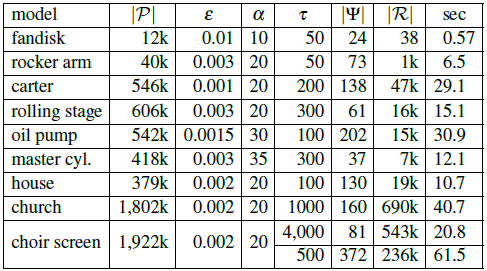
\includegraphics[width=0.7\textwidth]{Shape_Detection/schnabel-performance.png}
	\caption{The original statistics by Schnabel et. al\cite{schnabel-2007-efficient} on processed models. $\epsilon$ is given as ration of maximum bounding box with. Results have been averaged over 5 runs and rounded.}
	\label{table:schnabel_performance}
\end{table}

Table \ref{table:schnabel_performance} describes the statistical results obtained by Schnabel et. al\cite{schnabel-2007-efficient} for different models. $|P|$ is the number of points, $\epsilon$ the distance threshold, $\alpha$ the maximum normals deviation, $\tau$ is the minimum number of support points, $\|Psi|$ the number of shapes found, $|R|$ the number of RANSAC iterations. It can be seen that for small a small number of points and weaker constraints the algorithm returns plausible results within a fraction of a second. We utilize this feature the detect shapes in our application for small regions at a time to give immediate feedback to the user. 


\section{Selecting Candidate Nodes}
\label{sec:candidateNodes}
To select a proper candidate node from the octree, a node must fulfill the following constraints: 
\begin{itemize}
	\item The node must currently be rendered and visible to the user. 
	\item The node must contain at least $n$ points, the same amount used as minimal support point count for shape detection
	\item The node must not already contain detected shapes
\end{itemize}

Since this interaction is guided by the user, it makes sense that the user only interacts with what is presented on screen. Therefore the node must currently be rendered and visible. In order to eliminate overhead for the shape detection, the node must have enough points to at least fit one shape, otherwise it is ignored. Lastly, the shape detection algorithm works under the probabilistic assumption that all shapes were found, once it terminates. Therefore, nodes that already contain detected shapes are ignored as well. 
\\
The shape detection is guided by the user's cursor position. 
A raycast is performed, in order to select nodes that intersect with the cursor. 
The ray is constructed from the cursor's position on the near plane $p$ and the vector pointing from the camera to $p$. This ray is referred to as pick ray. 
An octree is an ideal data structure to perform a raycast. If the parent does not intersect the ray, neither will the children. This can be used to accelerate the process and prematurely eliminate nodes. The raycast on the octree can be performed with logarithmic cost. The raycast collects all nodes that intersect the pick ray. 

To choose the most suitable node as candidate node we eliminate all nodes from the raycast result that do not fulfill the previous constraints. For all remaining nodes a key is created from the LoD-level and the projected distance to the nearplane. The LoD-level is larger the smaller the node is and the more detail it contains. This heuristic favors nodes with larger LoD-level so that the user receives geometric information for the most detailed parts that he is currently exploring. The projected nearplane distance is used to select between nodes with the same LoD-level. The node closest to the nearplane is favored Algorithm \ref{alg:candidateNodeHeuristic} showcases the selection heuristic that is executed for each intersecting node that intersects the pick ray. 




\section{Refitting}
\label{sec:Refitting}